\section{Análisis}

\begin{frame}{Reglas de negocio}
	\begin{enumerate}[label*=RN\arabic*]
		
		\item El estado de una celda en el tiempo $t + 1$ depende únicamente de su estado actual y de los estados de sus vecinos.

		\item Para iniciar la simulación es necesario que el conjunto de estados, la topología de la vecindad, la condición de frontera y la función de transición hayan sido definidas. 
		
		\item Cuando la simulación está en curso, no se puede cambiar el conjunto de estados, la topología de la vecindad ni la función de transición.
		
		\item El usuario puede manipular el estado de una célula y la condición de frontera en tiempo de ejecución.
	
	\end{enumerate}
\end{frame}

\begin{frame}{Reglas de negocio}
	\begin{enumerate}[label*=RN\arabic*]
		
		\setcounter{enumi}{4}
		
		\item Los datos importados deben cumplir con el formato definido por el sistema para garantizar su correcta interpretación.
		
		\item Los datos exportados deben conservar el mismo formato que los datos importados.
		
		\item El usuario puede pausar, detener, reanudar o retroceder la simulación sin pérdida de información. 
		
		\item Solo se permite una simulación activa por sesión.
		
	\end{enumerate}
\end{frame}


\begin{frame}{Requisitos funcionales}
	\begin{enumerate}[label=RF\arabic*.]
		
		\item El sistema debe mostrar una cuadrícula regular y finita que represente el espacio celular.
		
		\item El sistema debe permitir al usuario interactuar con el espacio celular, asignando o modificando los estados de las celdas.
		
		\item El sistema debe permitir al usuario definir el conjunto de estados, la topología de la vecindad local y las condiciones de frontera del espacio celular.
		
		\item El sistema debe permitir la evolución del espacio celular mediante un único paso o de forma continua, ajustando la velocidad de actualización según las capacidades computacionales del sistema.		
	\end{enumerate}
	
\end{frame}

\begin{frame}{Requisitos funcionales}
	\begin{enumerate}[label=RF\arabic*.]
		
		\setcounter{enumi}{4}
		
		\item El sistema debe permitir la importación y exportación de configuraciones y evoluciones del espacio celular.
		
		\item El sistema debe permitir al usuario establecer la función de transición de manera manual.
		
		\item El sistema debe permitir configurar la red neuronal para imitar el comportamiento de una evolución señalada.
		
		\item El sistema debe entrenar una red neuronal dados los parámetros del usuario y la evolución que desea replicar.
		
	\end{enumerate}
	
\end{frame}

\begin{frame}{Diagrama de casos de uso}
	\begin{figure}[H]
		\centering
		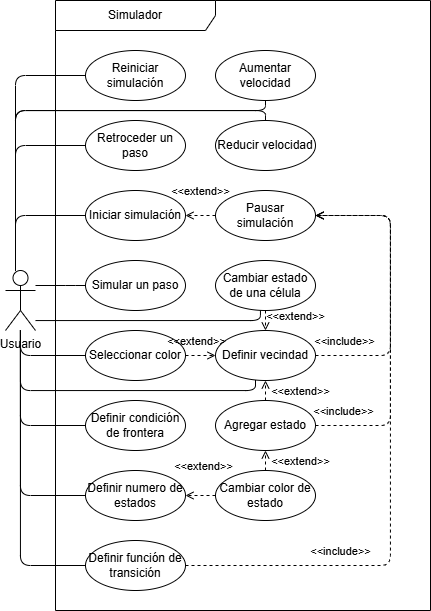
\includegraphics[width=0.3\linewidth]{images/uml_ucd.png}
		\caption{Diagrama de casos de uso}
		\label{fig:uml_ucd}
	\end{figure}
\end{frame}



